\section{System Overview}\label{ch:2}

\subsection{High-level architecture}

A submission flows through seven tiers:

\begin{figure}[htbp]
  \centering
  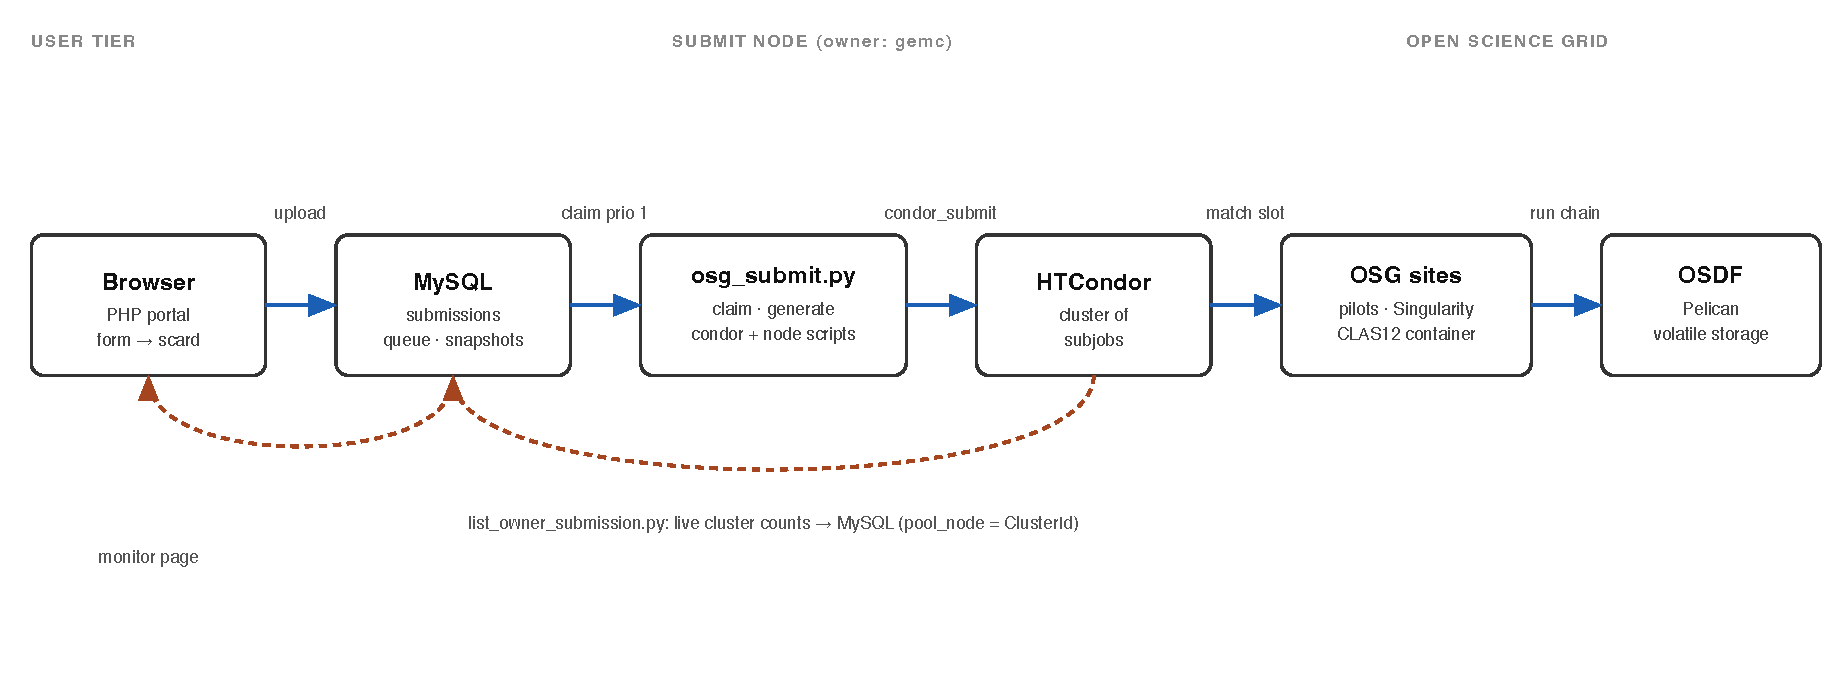
\includegraphics[width=\textwidth]{figures/fig1_architecture}
  \caption{simGrid high-level architecture. A submission flows browser $\rightarrow$ PHP portal $\rightarrow$ MySQL $\rightarrow$ submit node $\rightarrow$ HTCondor $\rightarrow$ OSG sites $\rightarrow$ OSDF. The browser never contacts HTCondor or the OSG directly; the submit node runs everything under the single shared owner \texttt{gemc}.}
  \label{fig:architecture}
\end{figure}

The browser never talks to HTCondor or the OSG directly. The PHP portal writes the request into MySQL; a periodically-run submission engine on the submit node claims requests one at a time, generates the HTCondor and worker-node scripts, and submits a cluster; the OSG runs the subjobs in the CLAS12 container and streams output to OSDF. Monitoring reads live HTCondor state and joins it back to MySQL for display.

\subsection{Component inventory and responsibilities}

\begin{itemize}
  \item \textbf{2.2.1 Web portal (\texttt{web\_\allowbreak{}portal/\allowbreak{}}, PHP + \texttt{main.\allowbreak{}js}).} Renders the submission forms, validates and caps user input in the browser, writes the scard, and invokes the uploader. Pages: \texttt{index}, \texttt{type1}, \texttt{type2}, \texttt{monitor}, \texttt{fairshare}, \texttt{osgStats}, \texttt{about}.
  \item \textbf{2.2.2 MySQL submission database (\texttt{CLAS12OCR} / \texttt{CLAS12TEST}).} The single source of truth for submissions, users, generated artifacts, snapshots, and both the pending-queue priority and cluster bookkeeping.
  \item \textbf{2.2.3 Submission engine (\texttt{osg\_\allowbreak{}submit.\allowbreak{}py}).} Claims the next pending request, parses its scard, stages a per-submission directory, generates the HTCondor card and nodescript, and runs \texttt{condor\_\allowbreak{}submit}.
  \item \textbf{2.2.4 Generators (\texttt{generators/\allowbreak{}condor/\allowbreak{}}, \texttt{generators/\allowbreak{}bash/\allowbreak{}}).} Pure functions that assemble the HTCondor submit file (nine sections) and the worker-node \texttt{nodescript.\allowbreak{}sh} (self-documenting steps).
  \item \textbf{2.2.5 Worker-node runtime (\texttt{nodescript.\allowbreak{}sh} + \texttt{functions.\allowbreak{}sh}).} The script that actually runs on each OSG slot: environment setup, input staging, GEMC, merging, denoising, reconstruction, DST, and upload.
  \item \textbf{2.2.6 Priority subsystems (\texttt{db\_\allowbreak{}io/\allowbreak{}priority\_\allowbreak{}submissions.\allowbreak{}py}, \texttt{condor\_\allowbreak{}io/\allowbreak{}run\_\allowbreak{}priority\_\allowbreak{}map.\allowbreak{}py}).} The pending-queue calculator (writes \texttt{submissions.\allowbreak{}priority}) and the runtime balancer (writes \texttt{JobPrio}).
  \item \textbf{2.2.7 Monitoring, snapshotting, and completion (\texttt{condor\_\allowbreak{}io/\allowbreak{}list\_\allowbreak{}owner\_\allowbreak{}submission.\allowbreak{}py}, \texttt{db\_\allowbreak{}io/\allowbreak{}mark\_\allowbreak{}completed\_\allowbreak{}submissions.\allowbreak{}py}, \texttt{stats/\allowbreak{}}).} Build the submissions table, snapshot it, detect completion, and produce long-term statistics.
\end{itemize}

\subsection{External dependencies and services}

\begin{itemize}
  \item \textbf{CVMFS} delivers the CLAS12 software modules and the Singularity image catalogue to every worker node.
  \item \textbf{Singularity/Apptainer} provides the \texttt{jeffersonlab/\allowbreak{}clas12software} container in which every job runs.
  \item \textbf{Pelican / OSDF} is the data federation used to read LUND input and write HIPO output; access is authenticated with a short-lived OAuth bearer token.
  \item \textbf{JLab volatile storage} (\texttt{/\allowbreak{}volatile/\allowbreak{}clas12/\allowbreak{}}, mirrored on OSDF) holds LUND inputs and receives outputs.
  \item \textbf{RCDB / SQLite} supplies run-dependent conditions consulted during reconstruction.
\end{itemize}

\subsection{Production vs. development environments}

Two parallel environments exist. Production uses the \texttt{CLAS12OCR} database, the \texttt{production} container tag, and the shared owner \texttt{gemc}. Development (\texttt{-\allowbreak{}-\allowbreak{}devel}) uses the \texttt{CLAS12TEST} database and the \texttt{devel} container tag; the portal also detects a development URL and switches banners and targets accordingly (\texttt{common.\allowbreak{}php}). This separation allows script and pipeline changes to be validated against reference submissions (Chapter 15) before reaching production.

\subsection{End-to-end data flow narrative}

A user opens \texttt{type1.\allowbreak{}php}, chooses a configuration, generator, fields, vertex handling, event/job counts, background-merging option, and output type, and clicks Submit. \texttt{submit\_\allowbreak{}type1.\allowbreak{}php} assembles a scard and execs \texttt{db\_\allowbreak{}io/\allowbreak{}upload\_\allowbreak{}submission.\allowbreak{}py}, which ensures the user exists, inserts one \texttt{submissions} row with \texttt{run\_\allowbreak{}status =\allowbreak{} 'Not Submitted'}, and appends it to the contiguous \texttt{1.\allowbreak{}.\allowbreak{}N} pending queue under a database lock. The fair-share calculator later reorders that queue. On the submit node, \texttt{osg\_\allowbreak{}submit.\allowbreak{}py} runs (from cron), checks capacity, claims the priority-1 row (marking it \texttt{Processing}), parses its scard, stages \texttt{\textasciitilde{}/\allowbreak{}osgOutput/\allowbreak{}<user>/\allowbreak{}job\_\allowbreak{}<id>/\allowbreak{}}, generates \texttt{clas12.\allowbreak{}condor} and \texttt{nodescript.\allowbreak{}sh}, and runs \texttt{condor\_\allowbreak{}submit}. The row becomes \texttt{Submitted to OSG} with its \texttt{ClusterId} recorded in \texttt{pool\_\allowbreak{}node}. HTCondor matches each subjob onto an OSG slot; the worker node runs the full chain and uploads the HIPO output to the user's OSDF namespace. Monitoring joins live cluster counts back to MySQL, snapshots the table, and eventually marks the submission \texttt{Completed}.
